% Created 2015-03-23 Mon 14:34
\documentclass[11pt]{article}
\usepackage[utf8]{inputenc}
\usepackage{lmodern}
\usepackage[T1]{fontenc}
\usepackage{fixltx2e}
\usepackage{graphicx}
\usepackage{longtable}
\usepackage{float}
\usepackage{wrapfig}
\usepackage{rotating}
\usepackage[normalem]{ulem}
\usepackage{amsmath}
\usepackage{textcomp}
\usepackage{marvosym}
\usepackage{wasysym}
\usepackage{amssymb}
\usepackage{amsmath}
\usepackage[version=3]{mhchem}
\usepackage[numbers,super,sort&compress]{natbib}
\usepackage{natmove}
\usepackage{url}
\usepackage{minted}
\usepackage{underscore}
\usepackage[linktocpage,pdfstartview=FitH,colorlinks,
linkcolor=blue,anchorcolor=blue,
citecolor=blue,filecolor=blue,menucolor=blue,urlcolor=blue]{hyperref}
\usepackage{attachfile}
\usepackage[left=1in, right=1in, top=1in, bottom=1in, nohead]{geometry}
\usepackage{hyperref}
\usepackage{setspace}
\usepackage[labelfont=bf]{caption}
\usepackage{amsmath}
\usepackage{enumerate}
\usepackage[parfill]{parskip}
\author{Prateek Mehta, William F. Schneider}
\date{\textit{<2015-03-24 Tue>}}
\title{Computational Chemistry Laboratory IV (CBE 60547)}
\begin{document}

\maketitle


\section{Common sources of error from the last homework!}
\label{sec-1}

Mostly everyone did a good job on the last homework. There were a few common mistakes, listed below.

\begin{itemize}
\item Not checking if results make sense
\begin{itemize}
\item e.g. if the calculation took only one relaxation step, the geometry is probably not converged
\item always a good idea to check with your input files and output files
\end{itemize}

\item Bond energies 
\begin{itemize}
\item e.g. for oxygen, bond energy is $E_{O_{2}} + E_{ZPE} - 2E_{O}$
\item absolute DFT energies are meaningless!
\end{itemize}

\item Use consistent planewave cutoffs when comparing different calculations.

\item Typos, spelling mistakes, forgetting to change directory names

\item \texttt{jasp} is built for continuation runs
\begin{itemize}
\item reads the input parameters from the files in the directory
\item jobs are resubmitted if parameters are added or updated
\item If parameters are removed, the original parameters written in your directory \textbf{will stay!}
\item Changing atoms objects after running the code is a bad idea! (\texttt{jasp} got updated to raise errors if you do this)
\end{itemize}

\item Those not submitting org generated pdfs, make sure you inculde enough information (incar parameters, pseudopotentials used, etc.) to make your calculations reproducible
\end{itemize}


\section{Bulk Systems}
\label{sec-2}

\subsection{Creating a bulk system}
\label{sec-2-1}

There are a few different functions built into ase that let's you create simple bulk systems. The one we will use is \href{ase.lattice.bulk}{ase.lattice.bulk}. Let us consider how to construct an fcc structure. You can either create the primitive cell (default), a orthorhombic cell, or a cubic cell. Note these will have different unit cell sizes and different number of atoms, which will affect the computational cost of your simulation. 

\begin{minted}[frame=lines,fontsize=\scriptsize,linenos]{python}
from ase.lattice import bulk
from jasp import *
import matplotlib.pyplot as plt
from ase.visualize import view

# a is the lattice constant in Angstroms
Pd_cubic = bulk('Pd', 'fcc', a=3.89, cubic=True) 
view(Pd_cubic)
print Pd_cubic

Pd_ortho = bulk('Pd', 'fcc', a=3.89, orthorhombic=True)
view(Pd_ortho)
print Pd_ortho

Pd_primitive = bulk('Pd', 'fcc') # if a is not specified, default experimental value is used.
view(Pd_primitive)
print Pd_primitive
\end{minted}

\begin{verbatim}
Atoms(symbols='Pd4', positions=..., cell=[3.89, 3.89, 3.89],
      pbc=[True, True, True])
Atoms(symbols='Pd2', positions=..., cell=[2.75064537881567,
      2.75064537881567, 3.89], pbc=[True, True, True])
Atoms(symbols='Pd', positions=..., cell=[[0.0, 1.945, 1.945], [1.945,
      0.0, 1.945], [1.945, 1.945, 0.0]], pbc=[True, True, True])
\end{verbatim}

Calculations can be done in a similar way to what we performed in the last lab and homework, with a few additional parameters. The most important of these is the \emph{k}-point grid.

\subsection{A little bit about \emph{k}-points}
\label{sec-2-2}

For modeling bulk systems/surfaces, we need to specify a \emph{k}-point mesh. A few things to note:

\begin{itemize}
\item The accuracy (and cost) of your simulation usually goes up with increasing the \emph{k}-point grid used.

\item In this lab (for demonstrative purposes only) a k-point grid of (8x8x8) has been used. We typically need to do a convergence study for \emph{k}-points, similar to the one we did for the planewave cutoff.

\item The number of \emph{k}-points required scales inversely with the size of the unit cell.

\item We will usually specify a parameter \verb~kpts=(k1,k2,k3)~ in \texttt{jasp}, which creates a \texttt{KPOINTS} file that tells \texttt{VASP} to \href{http://cms.mpi.univie.ac.at/vasp/vasp/Automatic_k_mesh_generation.html}{automatically create a Monkhorst-Pack k-mesh.}

\item Metals (conductors) generally require more \emph{k}-points than insulators to reach the same level of convergence.
\end{itemize}

\subsection{Optimizing lattice constants - Equations of State}
\label{sec-2-3}

\subsubsection{Energies vs. Lattice Constants}
\label{sec-2-3-1}

\texttt{ase} by default uses the experimental lattice constants (if known). Our computationally calculated lattice constants will usually be slightly different, depending on the exchange-correlation functional used. Let us consider a series of lattice constants, to find out which one minimizes the total energy.

\begin{minted}[frame=lines,fontsize=\scriptsize,linenos]{python}
from ase.lattice import bulk
from jasp import *
import numpy as np
import matplotlib.pyplot as plt
from ase.utils.eos import EquationOfState

# Generate an array of 7 points 10% around 3.89 angstroms
A = np.linspace(3.89 * 0.9, 3.89 * 1.1, 7) 

energies = []

ready = True
for a in A:
    # We will use the cubic cell for simplicity
    Pd_cubic = bulk('Pd', 'fcc', a=a, cubic=True)
    
    with jasp('EOS/Pd-a-{0:1.2f}'.format(a),
              xc='PBE',
              encut=400,
              ismear=1, # Use MP smearing for metals
              kpts=(8,8,8), #A much larger grid is reqd to be accurate!
              atoms=Pd_cubic) as calc:
        try:
            calc.calculate()
            energies.append(Pd_cubic.get_potential_energy())
                                       
        except(VaspSubmitted, VaspQueued):
            ready = False

if not ready:
    import sys; sys.exit()              

plt.plot(A, energies, 'bo-')
plt.xlabel('Lattice constant ($\AA$)')
plt.ylabel('Total energy (eV)')
plt.savefig('images/Pd-fcc-lattice.png')
plt.show()
\end{minted}

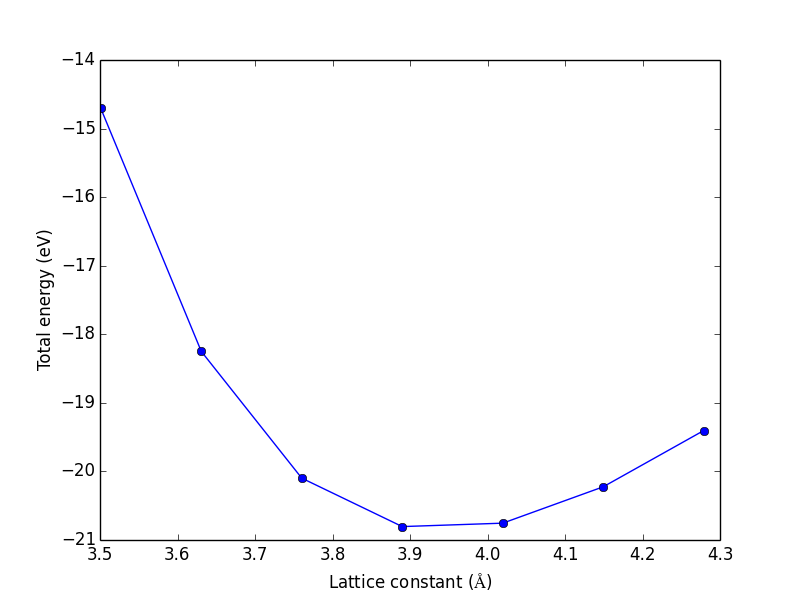
\includegraphics[width=.9\linewidth]{./images/Pd-fcc-lattice.png}


\subsubsection{Fitting to an Equation of State}
\label{sec-2-3-2}

To find the 'optimal' lattice constant we need to fit our data to an \href{http://gilgamesh.cheme.cmu.edu/doc/software/jacapo/appendices/appendix-eos.html}{equation of state}, which describes the energy as a function of volume. The Murnaghan or Birch-Murnaghan EOS is commonly used. Let us use \href{ase.utils.eos}{ase.utils.eos} to fit the data we calculated above to the Birch-Murnaghan EOS.

\begin{minted}[frame=lines,fontsize=\scriptsize,linenos]{python}
from jasp import *
import numpy as np
import matplotlib.pyplot as plt
from ase.utils.eos import EquationOfState

# Generate an array of 7 points 10% around 3.89
A = np.linspace(3.89 * 0.9, 3.89 * 1.1, 7) 

energies = []
volumes = []

for a in A:

    with jasp('EOS/Pd-a-{0:1.2f}'.format(a)) as calc:
        atoms = calc.get_atoms()
        energies.append(atoms.get_potential_energy())
        volumes.append(atoms.get_volume())

eos = EquationOfState(volumes, energies, eos='birchmurnaghan')
v0, e0, b = eos.fit()
a0 = v0 ** (1/3.)
eos.plot(filename='images/Pd-EOS.png', show=True)

print 'Minimum Energy = {0:1.3f} eV'.format(e0)
print 'Optimal Volume = {0:1.3f} cubic angstroms'.format(v0)
print 'Optimal lattice constant = {0:1.3f} angstroms'.format(a0)
\end{minted}

\begin{verbatim}
Minimum Energy = -20.933 eV
Optimal Volume = 60.782 cubic angstroms
Optimal lattice constant = 3.932 angstroms
\end{verbatim}

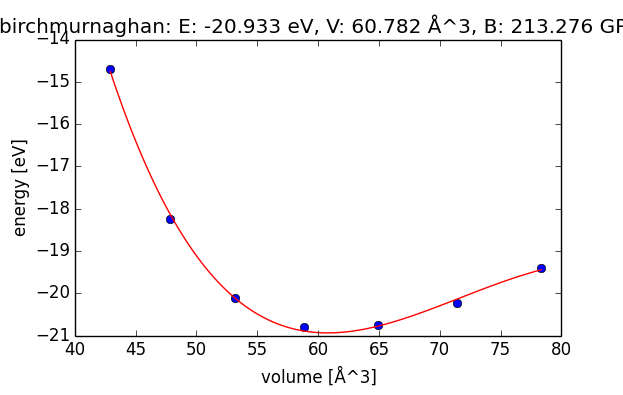
\includegraphics[width=.9\linewidth]{./images/Pd-EOS.png}


\section{Surfaces}
\label{sec-3}

\subsection{Creating a surface}
\label{sec-3-1}

\texttt{ase} provides functions to create surfaces too. Surfaces are layers of atoms formed by cleaving the bulk structure in a given direction. In our models, we add vacuum in the direction perpendicular to the surface. Thus, the atoms are finite in the direction perpendicular to the surface, but infinite in the other two directions. Here is an example of how to make a surface.

\begin{minted}[frame=lines,fontsize=\scriptsize,linenos]{python}
from ase.lattice.surface import fcc111
from jasp import *
from ase.visualize import view
from ase.constraints import FixAtoms

a = 3.932 # Optimal lattice constant from EOS

# Create a surface with 3 unit cells in x and y
# 3 layers deep
atoms = fcc111('Pd', size=(2,2,3), vacuum=10.0, a=a)
view(atoms)
for atom in atoms:
    print atom
write('images/Pd-slab.png', atoms, rotation='90x', show_unit_cell=2)
\end{minted}

\begin{verbatim}
Atom('Pd', [1.3901719318127526, 0.8026161390519545, 10.0], tag=3, index=0)
Atom('Pd', [4.1705157954382575, 0.8026161390519545, 10.0], tag=3, index=1)
Atom('Pd', [2.7803438636255051, 3.210464556207818, 10.0], tag=3, index=2)
Atom('Pd', [5.5606877272510102, 3.210464556207818, 10.0], tag=3, index=3)
Atom('Pd', [0.0, 1.605232278103909, 12.270141258453609], tag=2, index=4)
Atom('Pd', [2.7803438636255051, 1.605232278103909, 12.270141258453609], tag=2, index=5)
Atom('Pd', [1.3901719318127523, 4.013080695259772, 12.270141258453609], tag=2, index=6)
Atom('Pd', [4.1705157954382575, 4.013080695259772, 12.270141258453609], tag=2, index=7)
Atom('Pd', [0.0, 0.0, 14.540282516907219], tag=1, index=8)
Atom('Pd', [2.7803438636255051, 0.0, 14.540282516907219], tag=1, index=9)
Atom('Pd', [1.3901719318127526, 2.4078484171558636, 14.540282516907219], tag=1, index=10)
Atom('Pd', [4.1705157954382575, 2.4078484171558636, 14.540282516907219], tag=1, index=11)
\end{verbatim}

The tag on the atom indicates which layer of the surface it is in.

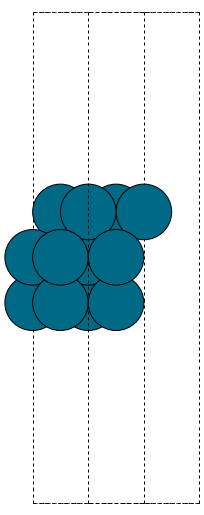
\includegraphics[width=205bp]{./images/Pd-slab.png}

We can see that there are actually two surfaces, one in the top layer and one at the bottom layer. Surface atoms will tend to contract toward the bulk due to decreased coordination. 

To simulate bulk like behavior in regions away from the surface, we can do two things:

\begin{itemize}
\item increase the number of layers in the slab (requires many atoms, large cost)

\item Constrain(freeze) the the bottom layer(s) in their bulk positions (common, lower cost). The bottom layer is now representative of bulk behavior.
\end{itemize}


\subsection{Surface calculations}
\label{sec-3-2}

Let us now optimize the geometry of our surface. \textbf{Note that only one \emph{k}-point is required in the direction perpendicular to the surface.}

\begin{minted}[frame=lines,fontsize=\scriptsize,linenos]{python}
from ase.lattice.surface import fcc111
from jasp import *
from ase.visualize import view
from ase.constraints import FixAtoms

JASPRC['queue.nprocs'] = 8
JASPRC['queue.q'] = 'short'

a = 3.932 # Optimal lattice constant from EOS
atoms = fcc111('Pd', size=(2,2,3), vacuum=10.0, a=a)

constraint = FixAtoms(mask=[atom.tag >= 3 for atom in atoms])
atoms.set_constraint(constraint)

with jasp('surfaces/Pd-slab-relaxed',
          xc='PBE',
          ismear=1,
          kpts=(8, 8, 1),
          encut=400,
          ibrion=2, # Conjugate Gradient
          nsw=20, # relaxation steps
          atoms=atoms) as calc:
    calc.calculate()
    print calc
\end{minted}

\begin{verbatim}
: -----------------------------
  VASP calculation from /afs/crc.nd.edu/user/p/pmehta1/computational-chemistry/Lab4/surfaces/Pd-slab-relaxed
  converged: True
  Energy = -58.019294 eV

  Unit cell vectors (angstroms)
        x       y     z      length
  a0 [ 5.561  0.000  0.000] 5.561
  a1 [ 2.780  4.816  0.000] 5.561
  a2 [ 0.000  0.000  24.540] 24.540
  a,b,c,alpha,beta,gamma (deg):5.561 5.561 24.540 90.0 90.0 90.0
  Unit cell volume = 657.154 Ang^3
  Stress (GPa):xx,   yy,    zz,    yz,    xz,    xy
             0.012  0.012  0.000-0.000 -0.000 -0.000
 Atom#  sym       position [x,y,z]tag  rmsForce constraints
   0    Pd  [1.390      0.803     10.000]  3   0.00      F F F
   1    Pd  [4.171      0.803     10.000]  3   0.00      F F F
   2    Pd  [2.780      3.210     10.000]  3   0.00      F F F
   3    Pd  [5.561      3.210     10.000]  3   0.00      F F F
   4    Pd  [5.561      1.605     12.270]  2   0.04      T T T
   5    Pd  [2.780      1.605     12.270]  2   0.04      T T T
   6    Pd  [6.951      4.013     12.270]  2   0.04      T T T
   7    Pd  [4.171      4.013     12.270]  2   0.04      T T T
   8    Pd  [0.000      0.000     14.548]  1   0.02      T T T
   9    Pd  [2.780      0.000     14.548]  1   0.02      T T T
   10   Pd  [1.390      2.408     14.548]  1   0.02      T T T
   11   Pd  [4.171      2.408     14.548]  1   0.02      T T T
--------------------------------------------------

INCAR Parameters:
-----------------
        nbands: 72
        ismear: 1
           nsw: 20
        ibrion: 2
         encut: 400.0
        magmom: None
          kpts: (8, 8, 1)
    reciprocal: False
            xc: PBE
           txt: -
         gamma: False

Pseudopotentials used:
----------------------
Pd: potpaw_PBE/Pd/POTCAR (git-hash: 04426435b178dfad58ed91b470847d50ff70b858)
\end{verbatim}

Note that Vasp is a little unintuitive. The constraint 'F' means frozen.

We can go back to the calculation directory and see how our surface relaxed with \verb~jaspsum -t~.



\subsection{Adding an Adsorbate}
\label{sec-3-3}

Now let us add an adsorbate on our surface. There are multiple places where it could adsorb. Here is a picture of a fcc(111) gold surface, showing the possible adsorption sites. 


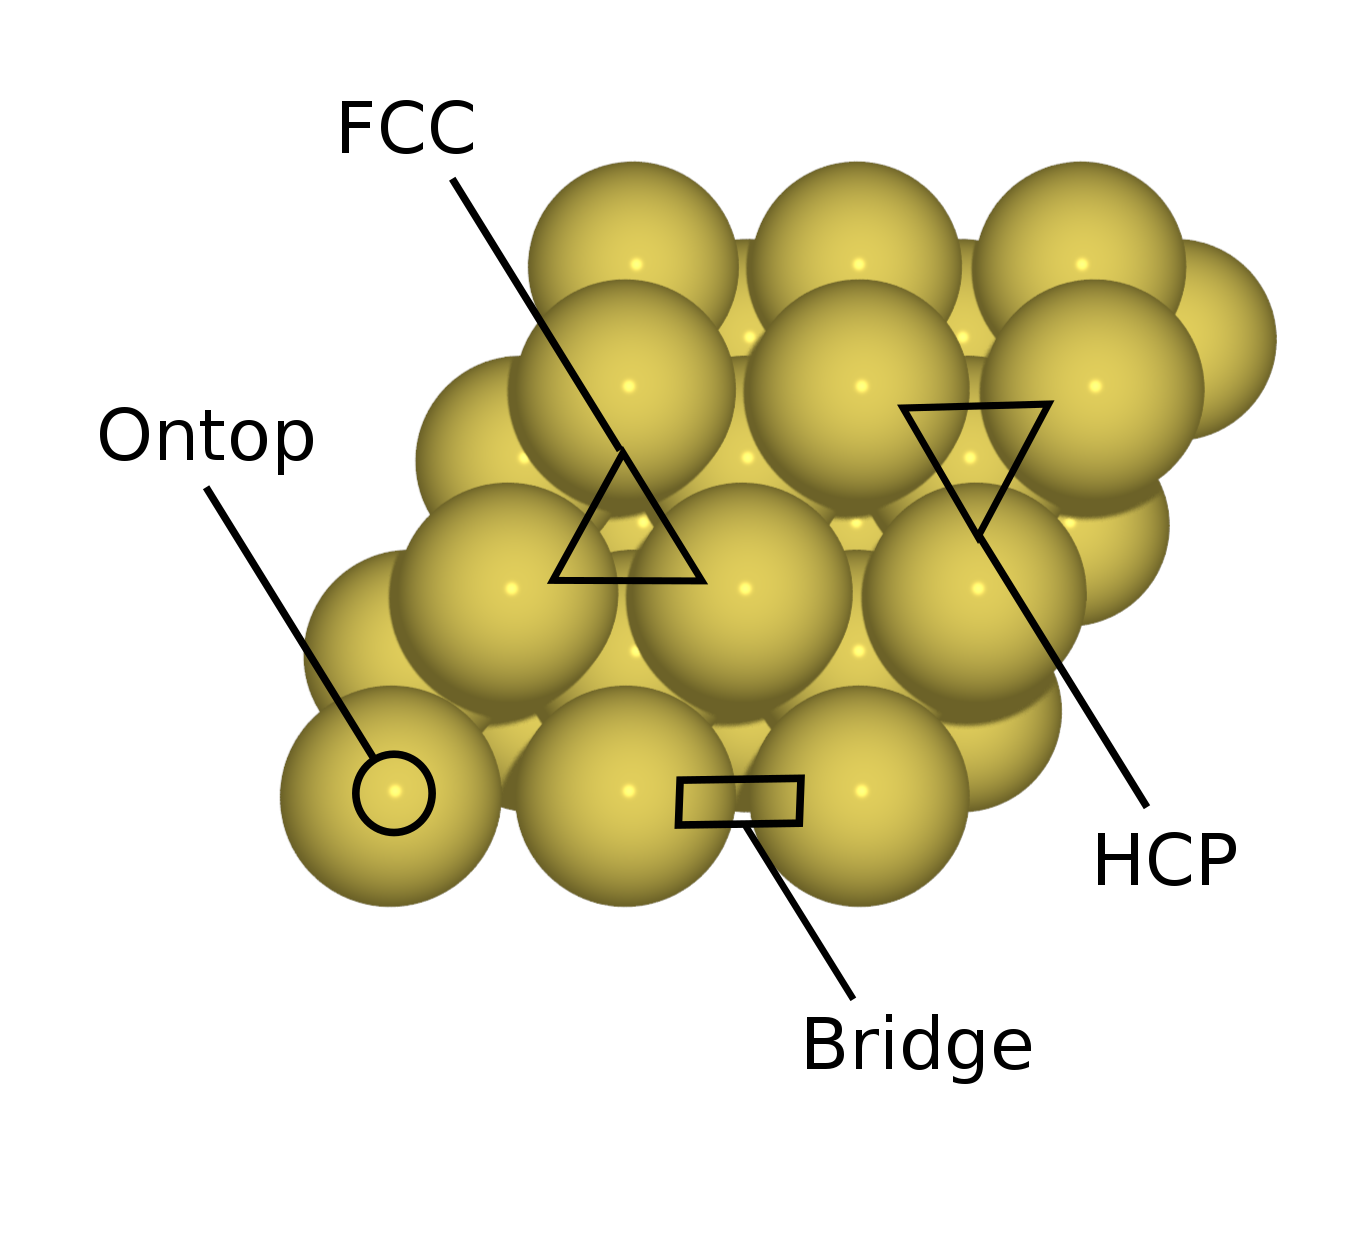
\includegraphics[width=.9\linewidth]{./images/Au-slab-sites.png}


Let's go back to our Pd surface and perform a calculation with an Oxygen adsorbate at the fcc site.

\begin{minted}[frame=lines,fontsize=\scriptsize,linenos]{python}
from ase.lattice.surface import fcc111, add_adsorbate
from jasp import *
from ase.visualize import view
from ase.constraints import FixAtoms

a = 3.932 # Optimal lattice constant from EOS
atoms = fcc111('Pd', size=(2,2,3), vacuum=10.0)

add_adsorbate(atoms, 'O', height=1.2, position='fcc')

# Note that constraints only work after adding the adsorbate
constraint = FixAtoms(mask=[atom.tag >= 3 for atom in atoms])
atoms.set_constraint(constraint)

# view(atoms)
with jasp('surfaces/O-on-Pd-fcc',
          xc='PBE',
          ismear=1,
          kpts=(8, 8, 1),
          encut=400,
          ibrion=2, # Conjugate Gradient
          nsw=20, # relaxation steps
          atoms=atoms) as calc:
    calc.calculate()
    print calc
    
write('images/Pd-slab-O-fcc.png', atoms, show_unit_cell=2)
\end{minted}

\begin{verbatim}
: -----------------------------
  VASP calculation from /afs/crc.nd.edu/user/p/pmehta1/computational-chemistry/Lab4/surfaces/O-on-Pd-fcc
  converged: True
  Energy = -64.436725 eV

  Unit cell vectors (angstroms)
        x       y     z      length
  a0 [ 5.501  0.000  0.000] 5.501
  a1 [ 2.751  4.764  0.000] 5.501
  a2 [ 0.000  0.000  24.492] 24.492
  a,b,c,alpha,beta,gamma (deg):5.501 5.501 24.492 90.0 90.0 90.0
  Unit cell volume = 641.919 Ang^3
  Stress (GPa):xx,   yy,    zz,    yz,    xz,    xy
             0.004  0.004  0.002-0.000 -0.000 -0.000
 Atom#  sym       position [x,y,z]tag  rmsForce constraints
   0    Pd  [1.375      0.794     10.000]  3   0.00      F F F
   1    Pd  [4.126      0.794     10.000]  3   0.00      F F F
   2    Pd  [2.751      3.176     10.000]  3   0.00      F F F
   3    Pd  [5.501      3.176     10.000]  3   0.00      F F F
   4    Pd  [5.505      1.586     12.288]  2   0.02      T T T
   5    Pd  [2.747      1.586     12.288]  2   0.02      T T T
   6    Pd  [6.877      3.970     12.405]  2   0.03      T T T
   7    Pd  [4.126      3.975     12.288]  2   0.02      T T T
   8    Pd  [-0.031    -0.018     14.660]  1   0.01      T T T
   9    Pd  [2.782     -0.018     14.660]  1   0.01      T T T
   10   Pd  [1.375      2.418     14.660]  1   0.01      T T T
   11   Pd  [4.126      2.382     14.541]  1   0.01      T T T
   12   O   [1.375      0.794     15.820]  0   0.02      T T T
--------------------------------------------------

INCAR Parameters:
-----------------
        nbands: 80
        ismear: 1
           nsw: 20
        ibrion: 2
         encut: 400.0
        magmom: None
          kpts: (8, 8, 1)
    reciprocal: False
            xc: PBE
           txt: -
         gamma: False

Pseudopotentials used:
----------------------
O: potpaw_PBE/O/POTCAR (git-hash: 592f34096943a6f30db8749d13efca516d75ec55)
Pd: potpaw_PBE/Pd/POTCAR (git-hash: 04426435b178dfad58ed91b470847d50ff70b858)
\end{verbatim}

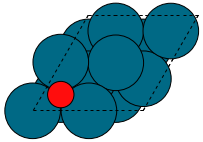
\includegraphics[width=2in]{./images/Pd-slab-O-fcc.png}



\subsection{Calculating adsorption energies}
\label{sec-3-4}

The adsorption energy is given by $E_{ads} = E_{surface+O} - E_{surface} - 0.5 E_{O_{2}}$. This can easily be calculated from the two calculations we performed and the O$_{\text{2}}$ calculation from the last homework.


\section{Density of States}
\label{sec-4}

It is possible to plot out the density of states (DOS) from \texttt{VASP} calculations. The density of states describes the number of states per interval of energy at each energy level that are available to be occupied (Wikipedia). 

\subsection{Total density of States}
\label{sec-4-1}

We can get the total density of states from an old DFT calculation without having to run a new calculation (Though the \texttt{VASP} manual recommends an additional run at ismear=-5). The DOS depends on the \emph{k}-point grid you choose.


Let's read in our calculation from our bulk Pd lattice constant studies.

\begin{minted}[frame=lines,fontsize=\scriptsize,linenos]{python}
from jasp import *
from ase.calculators.vasp import VaspDos
import matplotlib.pyplot as plt

with jasp('EOS/Pd-a-3.89') as calc:
    # Get the dos referenced at the fermi level
    dos = VaspDos(efermi=calc.get_fermi_level())
  
energies = dos.energy
dos = dos.dos

plt.plot(energies, dos, linewidth=2)
# Add a vertical line at the fermi level
plt.axvline(x=0, color='r', linestyle='--', linewidth=2)
plt.ylim(0,12)
plt.xlabel('energy (eV)')
plt.ylabel('DOS (arb. units)')
plt.savefig('images/Pd-bulk-dos.png')
plt.show()
\end{minted}

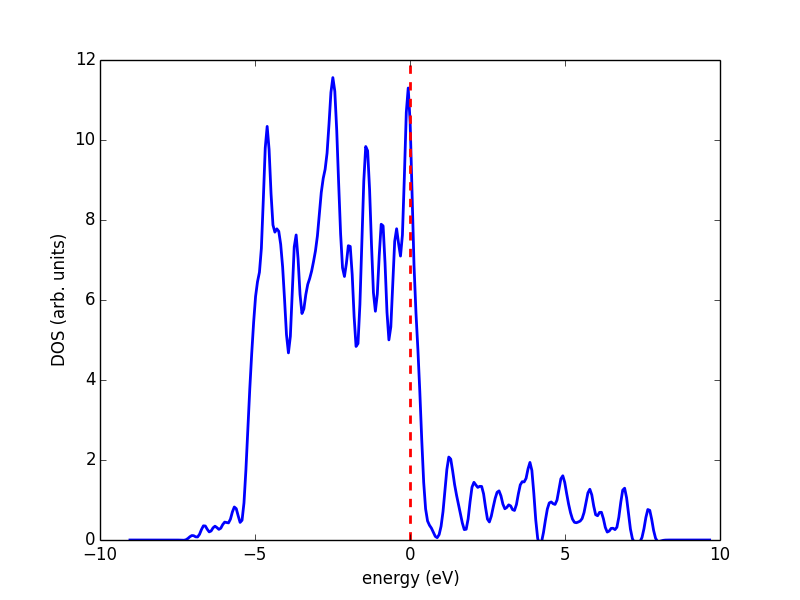
\includegraphics[width=.9\linewidth]{./images/Pd-bulk-dos.png}

States to the left of the fermi level (indicated by the red line) are the occupied states.


\subsection{Atom-projected density of states}
\label{sec-4-2}

To figure out which density of states belong to which atoms in a molecule, we need to perform an additional calculation. We can compute the atom-projected density of states (ADOS), which is done by projecting the wave function onto localized atomic orbitals. These are only a qualitative representation of the orbitals, because the atoms will often form molecular orbitals, hybridize, etc. 

In \texttt{VASP} we can specify an \href{http://cms.mpi.univie.ac.at/wiki/index.php/RWIGS}{RWIGS} parameter, which is radius around the atom at which to cutoff the projection. The choice of RWIGS is somewhat arbitrary, one can choose the ionic radius of an atom, or a value that minimizes overlap of neighboring spheres. Another way to calculate the ADOS is by specifying the \href{http://cms.mpi.univie.ac.at/vasp/vasp/LORBIT.html}{LORBIT} parameter to be 10 or 11, but this only works for PAW potentials (this is what we will use).

In transition metals, the s and p states are dispersed, and the only states that matter in terms of bonding are the d-states. Here is an example to plot the DOS projected on to the d states for clean Pd surface atoms.

\begin{minted}[frame=lines,fontsize=\scriptsize,linenos]{python}
from jasp import *
from ase.calculators.vasp import VaspDos
import matplotlib.pyplot as plt

# get the geometry the previous calculation
with jasp('surfaces/Pd-slab-relaxed') as calc:
    atoms = calc.get_atoms()

#Now submit a calculation for the ados
with jasp('surfaces/Pd-ados',
          xc='PBE',
          ismear=1,
          kpts=(8, 8, 1),
          encut=400,
          lorbit=10,
          atoms=atoms) as calc:
    calc.calculate()

    ados = VaspDos(efermi=calc.get_fermi_level())
    energies = ados.energy
    # Atom index 10 is a surface atom (tag=1)
    print atoms[10]
    d_dos = ados.site_dos(10, 'd')

    plt.plot(energies, d_dos, lw=2)

plt.axvline(lw=2, ls='--', color='r')
plt.ylim(0, 3.5)
plt.xlabel('energy (eV)')
plt.ylabel('DOS (arb. units)')
plt.savefig('images/Pd-ados.png')
plt.show()
\end{minted}

\begin{verbatim}
Atom('Pd', [1.3901719318127526, 2.4078484171558636, 14.548402978407839], tag=1, index=10)
\end{verbatim}

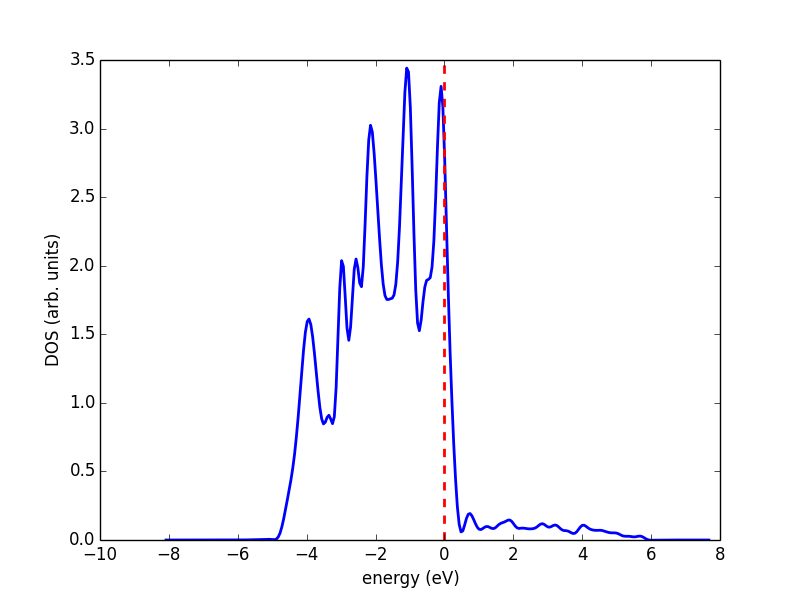
\includegraphics[width=.9\linewidth]{./images/Pd-ados.png}




\subsection{Adsorbate density of states}
\label{sec-4-3}

Now let us plot the density of states for the adsorbed O atom.

\begin{minted}[frame=lines,fontsize=\scriptsize,linenos]{python}
from jasp import *
import matplotlib.pyplot as plt

# get the geometry the previous calculation
with jasp('surfaces/O-on-Pd-fcc') as calc:
    atoms = calc.get_atoms()

JASPRC['queue.q'] = 'short'

#Now submit a calculation for the ados
with jasp('surfaces/O-on-Pd-fcc-ados',
          xc='PBE',
          ismear=1,
          kpts=(8, 8, 1),
          encut=400,
          lorbit=10,
          atoms=atoms) as calc:
    calc.calculate()

    O_ados = VaspDos(efermi=calc.get_fermi_level())
    energies = O_ados.energy
    # Plot the O ados
    # 12 is the index of the O atom
    s_dos = O_ados.site_dos(12, 's') 
    p_dos = O_ados.site_dos(12, 'p')
    plt.plot(energies, s_dos, label='O$_{s}$', lw=2)
    plt.plot(energies, p_dos, label='O$_{p}$', lw=2)    

# Now plot the clean surface ados for comparison
with jasp('surfaces/Pd-ados') as calc:
    ados = VaspDos(efermi=calc.get_fermi_level())
    energies = ados.energy
    
    d_dos = ados.site_dos(11, 'd')
    plt.plot(energies, d_dos, label='Pd$_{d}$', lw=2)
plt.xlim(-20, 8)
plt.ylim(0, 4)
plt.axvline(ls='-.', color='k', lw=2)
plt.xlabel('energy (eV)')
plt.ylabel('DOS (arb. units)')
plt.legend()
plt.savefig('images/adsorbate-dos.png')
plt.show()
\end{minted}

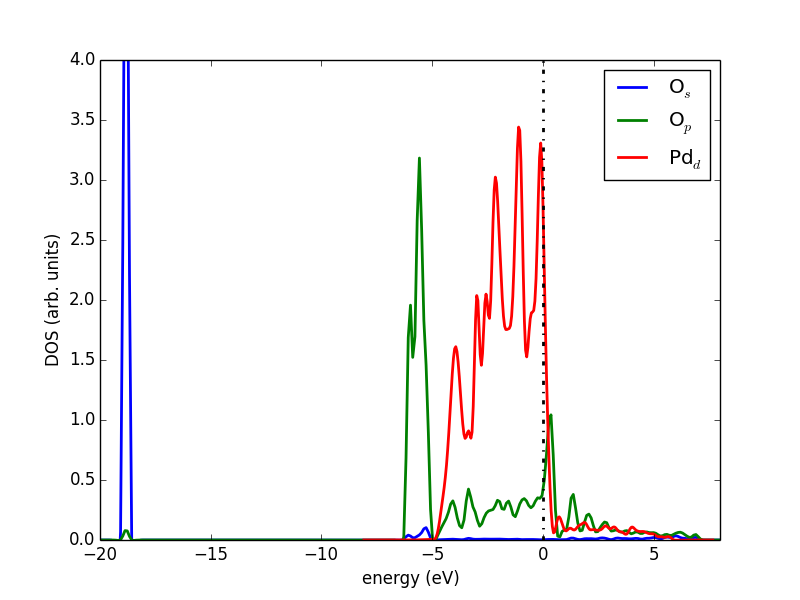
\includegraphics[width=.9\linewidth]{./images/adsorbate-dos.png}

The blue line indicates the Oxygen s-states. The two peaks of the green line left and right of the Pd d-band are the bonding and antibonding Oxygen p-states. Note that the antibonding peak is to the right of the fermi level, meaning that the antibonding states are unoccupied.
% Emacs 24.4.3 (Org mode 8.2.10)
\end{document}